So far we've seen several examples of rings which are subsets of other rings, like \(2\ZZ\) in \(\ZZ\) and \(\POWP{X}\) in \(\POW{X}\).
This suggests an alternative answer to the Construction Problem: take a \emph{subset} of an existing ring \(R\), and restrict the arithmetic to that subset.
There is a potential obstacle to making this work, though; given a subset \(S \subseteq R\) and two elements \(x,y \in S\), \emph{a priori} we expect their sum \(x+y\) and product \(xy\) to be in \(R\) but not necessarily in \(S\) -- see \autoref{fig:arithmetic-in-a-subset}.
\begin{figure}[h!]
\begin{center}
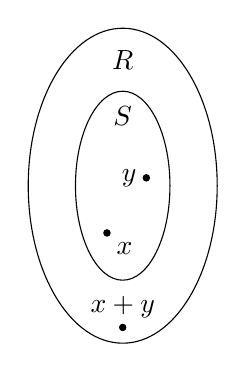
\begin{tikzpicture}[scale=0.4]
  \draw (0,0) ellipse (3 and 5);
  \node at (0,4) {\(R\)};
  \draw (0,0) ellipse (1.5 and 3);
  \draw [fill] (-0.5,-1.5) circle (0.1) node [below right] {\(x\)};
  \draw [fill] (0.75,0.25) circle (0.1) node [left] {\(y\)};
  \draw [fill] (0,-4.5) circle (0.1) node [above] {\(x+y\)};
  \node at (0,2.2) {\(S\)};
\end{tikzpicture}
\caption{Arithmetic in a subset \label{fig:arithmetic-in-a-subset}}
\end{center}
\end{figure}
This is a problem!
The plus and times on a ring must be \emph{closed}.
To avoid this, we single out exactly those subsets of \(R\) for which this does not happen.
That is, the subsets which are closed under the arithmetic on \(R\).

\begin{dfn}[Subring] \label{dfn:subring}
Let \(R\) be a ring and \(S \subseteq R\) a subset. We say that \(S\) is a \DefTerm{subring} of \(R\) if \(S\) is closed under the operations in \(R\). Specifically,
\begin{proplist*}
\item \(0_R \in S\), \label{dfn:subring:zero}
\item If \(x,y \in S\) then \(x+y \in S\), \label{dfn:subring:plus}
\item If \(x \in S\) then \(-x \in S\), and \label{dfn:subring:neg}
\item If \(x,y \in S\) then \(xy \in S\). \label{dfn:subring:times}
\end{proplist*}
If \(R\) is unital, we say that a subring \(S\) is \emph{unital} if in addition \(1_R \in S\). \index{unital!subring}
\end{dfn}

Of course we then have that

\begin{prop} \label{prop:subring-is-ring}
If \(R\) is a ring and \(S \subseteq R\) a subring, then \(S\) is itself a ring under the restricted operations on \(R\). If \(S\) is a unital subring of \(R\), then \(S\) is a unital ring.
\end{prop}

Using the definition, showing that a given sub\emph{set} of a ring is a sub\emph{ring} requires verifying four properties (or five if we want a unital subring). We have a slightly more efficient way to achieve this called the Subring Criterion.

\begin{prop}[Subring Criterion] \label{prop:subring-criterion}
Let \(S \subseteq R\) be a subset. Then \(S\) is a subring of \(R\) if and only if \(S\) is not empty and is closed under subtraction and multiplication. That is, \(S\) is a subring of \(R\) iff the following hold.
\begin{proplist*}
\item \(S \neq \varnothing\).
\item If \(x,y \in S\) then \(x-y \in S\).
\item If \(x,y \in S\) then \(xy \in S\).
\end{proplist*}
\end{prop}

\begin{proof}
First suppose \(S \subseteq R\) is a subring. Then \(S \neq \varnothing\), since \(0_R \in S\). Now if \(x,y \in S\), we have \(xy \in S\), and \(-y \in S\), and \(x + (-y) \in S\). So \(S\) satisfies the Subring Criterion. Conversely, suppose \(S\) satisfies the Subring Criterion. Since \(S\) is not empty, it contains an element \(s\), and since \(S\) is closed under subtraction we have \(0_R = s - s \in S\). Now if \(x\) is any element of \(S\) we have \(-x = 0_R - x \in S\), so that \(S\) is closed under negation. If \(x,y \in S\), then \(x+y = x-(-y) \in S\) and \(xy \in S\). Thus \(S\) is a subring of \(R\).
\end{proof}

The Subring Criterion is a slick way to show that a given subset of a ring is a subring. We have a yet more efficient way to characterize \emph{unital} subrings.

\begin{prop}[Unital Subring Criterion] \label{prop:unital-subring-criterion}
Let \(R\) be a unital ring. Then \(S \subseteq R\) is a unital subring if and only if \(1_R \in S\) and for all \(x,y,z \in S\), \(x-yz \in S\).
\end{prop}

\begin{proof}
Certainly if \(S\) is a unital subring of \(R\) then it satisfies the Unital Subring Criterion. Conversely, suppose \(S\) satisfies the Unital Subring Criterion. Now \(S\) is not empty since \(1_R \in S\). If \(x,y \in S\), then \(x-y = x - 1_R \cdot y \in S\), so that \(S\) is closed under subtraction. Now \(0_R = 1-R - 1_R1_R \in S\) and \(-x = 0_R - 1_R \cdot x \in S\) whenever \(x \in S\), so if \(x,y \in S\) we have \(xy = 0_R - (-x)y \in S\). By the Subring Criterion \(S\) is a subring of \(R\), and since \(1_R \in S\), it is a \emph{unital} subring of \(R\).
\end{proof}

\begin{examples}
\item \textbf{The zero subring.} Let \(R\) be any ring. The subset \(0 = \{0_R\} \subseteq R\) is a subring, called the \emph{zero subring}. (Show it!!)

\item Let \(R\) be a ring and \(k\) a positive integer, and define \(kR = \{ kr \mid r \in R \}\). Then \(kR \subseteq R\) is a subring, but is \emph{not} a unital subring. (@@@)

\item Let \(R\) be any ring and \(a \in R\). Then \(aR = \{ ar \mid r \in R \}\) is a subring of \(R\). (This is the content of \eref{exerc:aR-is-ring}.) Similarly, \(Ra = \{ ra \mid r \in R \}\) is a subring of \(R\). These subrings do not have to be the same!

\item If \(S_1, S_2 \subseteq R\) are (unital) subrings of \(R\), then \(S_1 \cap S_2 \subseteq R\) is also a (unital) subring of \(R\).
\end{examples}

There are two special subrings associated to every ring homomorphism: the \emph{image} and the \emph{kernel}.

\begin{prop}[Image and Kernel] \label{dfn:im-ker}
Let \(\varphi : R \rightarrow S\) be a ring homomorphism. Then we have the following.
\begin{proplist}
\item The set \[ \KER{\varphi} = \{ r \in R \mid \varphi(r) = 0 \}, \] called the \DefTerm{kernel} of \(\varphi\), is a subring of \(R\).
\item The set \[ \IM{\varphi} = \{ s \in S \mid s = \varphi(r)\ \mathrm{for\ some}\ r \in R \}, \] called the \DefTerm{image} of \(\varphi\), is a subring of \(S\).
\end{proplist}
\end{prop}

\begin{proof}
(@@@)
\end{proof}

The image of a homomorphism is everything in the codomain that ``gets hit'', while the kernel is everything in the domain that is ``sent to zero''. We can visualize these subsets as in \autoref{fig:im-ker}.

\begin{figure}[h!]
\begin{center}
\begin{tikzpicture}[scale=0.5]
  \draw (-7,0) ellipse (3 and 5);
  \node at (-7,4) {\(R\)};
  \draw [pattern=north west lines, pattern color=gray] (-7,0) ellipse (1.5 and 3);
  \draw [fill] (-7,-1) circle (0.1) node [below] {\(0_R\)};
  \node at (-7,1.5) {\(\KER{\varphi}\)};

  \draw (7,0) ellipse (3 and 5);
  \node at (7,4) {\(S\)};
  \draw [pattern=north west lines, pattern color=gray] (7,0) ellipse (1.5 and 3);
  \draw [fill] (7,-1) circle (0.1) node [below] {\(0_S\)};
  \node at (7,1.5) {\(\IM{\varphi}\)};

  \draw [gray] (-7,3) -- (7,-1);
  \draw [gray] (-7,-3) -- (7,-1);
  \draw [gray] (-7,5) -- (7,3);
  \draw [gray] (-7,-5) -- (7,-3);

  \node at (0,-5) {\(\varphi\)};
\end{tikzpicture}
\caption{The image and kernel of a homomorphism. \label{fig:im-ker}}
\end{center}
\end{figure}

The kernels of ring homomorphisms turn out to be very important, as we will see later in \autoref{chap:quot}. As a preview, we can think of homomorphisms \(\varphi : R \rightarrow S\) as projecting a ``shadow'' of \(R\) into \(S\) such that parts of \(R\) get collapsed down in the shadow. The kernel is the part of \(R\) which is collapsed to zero. As a consequence, the kernel measures how badly a homomorphism fails to be injective. Specifically:

\begin{prop} \label{prop:ker-zero}
A ring homomorphism \(\varphi\) is injective if and only if \(\KER{\varphi} = 0\).
\end{prop}

\begin{proof}
Suppose \(\varphi : R \rightarrow S\) is an injective homomorphism. If \(x \in \KER{\varphi}\), then (by definition) we have \(\varphi(x) = 0_S = \varphi(0_R)\). Since \(\varphi\) is injective, we have \(x = 0\). Thus \(\KER{\varphi} = 0\). Conversely, suppose \(\KER{\varphi} = 0\). Now suppose we have \(x,y \in R\) such that \(\varphi(x) = \varphi(y)\). Then \(\varphi(x - y) = \varphi(x) - \varphi(y) = 0\), so that \(x-y \in \KER{\varphi} = 0\). So \(x-y = 0\), and thus \(x = y\). Hence \(\varphi\) is injective.
\end{proof}

We have yet another way to characterize subrings: they are precisely the images of injective ring homomorphisms.

\begin{prop}
Let \(R\) be a ring and \(S \subseteq R\) a subset. The following are equivalent.
\begin{proplist}
\item \(S\) is a subring of \(R\).
\item There is an injective ring homomorphism \(\varphi : T \rightarrow R\) such that \(\IM{\varphi} = S\).
\end{proplist}
\end{prop}

Note that if \(\varphi : R \rightarrow S\) is an injective ring homomorphism, then we have \(R \cong \IM{\varphi}\). This allows us to think of \(R\) as a ``subring'' of \(S\), even though it isn't really, by identifying \(r \in R\) with \(\varphi(r) \in S\). At first this may seem like a trivial observation; we can think of \(R\) as sitting inside \(S\), okay. But suppose \(R\) is a particularly nasty or inconvenient ring to compute in, while \(S\) is very nice -- say, a ring of matrices or numbers. Then \(\varphi\) gives us a way to think of \(R\) in much more convenient terms. An injective mapping \(\varphi : R \rightarrow S\) is sometimes called a \emph{representation} of \(R\), as it literally allows us to ``represent'' elements of \(R\) by elements of \(S\).
\begin{titlebox}{The Representation Problem}
\begin{center}
What are all the representations \(\varphi : R \rightarrow S\) \\ of a ring \(R\) by rings \(S\) having property \(P\)?
\end{center}
\end{titlebox}
Property \(P\) here might be ``is a ring of sets'' or ``is a direct sum of rings of matrices''; typically, any property of rings which makes them particularly nice to compute in.



%---------%
\Exercises%
%---------%

\begin{exercise}
Let \(R = \ZZ\) and \(S \subseteq R\) the set of all prime integers. Show that \(S\) is \emph{not} a subring of \(R\).
\end{exercise}

\begin{exercise}
Let \(a, b > 1\) be relatively prime integers. Show that \(\ZZ/(a) \oplus \ZZ/(b) \cong \ZZ/(ab)\). (Hint: Use \eref{exerc:homs-from-zzn} and \ref{prop:ker-zero})
\end{exercise}

\begin{exercise}
Show that every subring of \(\ZZ\) is of the form \(k\ZZ\) for some \(k\). (@@@) is this true?
\end{exercise}

\begin{exercise}
Let \(R\) be a ring, and let \(e \in R\) be idempotent (that is, \(e^2 = e\)).
\begin{proplist*}
\item Show that \(eRe = \{ ere \mid r \in R \}\) is a subring of \(R\).
\item Show that as a ring, \(S = eRe\) is unital with \(1_S = e\).
\end{proplist*}
In particular, if \(R\) is a unital ring and \(e \neq 1_R\), then \(S\) is not a \emph{unital subring}, even though it is a \emph{subring which is unital}, since in a unital subring \(S\) we have \(1_S = 1_R\).
\end{exercise}

\begin{exercise}
Let \(R\) be a ring, and let \(\mathcal{S}\) be an arbitrary family of subrings of \(R\). Show that \(\bigcap_{S \in \mathcal{S}} S\) is a subring of \(R\).
\end{exercise}

\begin{dfn}[Triangular Matrix, Diagonal Matrix] \label{dfn:triangular-diagonal-matrix}
Let \(R\) be a ring. The set of \(2 \times 2\) \emph{upper triangular} matrices over \(R\) is defined to be \[ \UTMAT{2}{R} = \left\{ \begin{bmatrix} a_{11} & a_{12} \\ 0 & a_{22} \end{bmatrix} \mid a_{11}, a_{12}, a_{22} \in R \right\}. \] Similarly, the set of \(2 \times 2\) \emph{lower triangular} matrices is defined to be \[ \LTMAT{2}{R} = \left\{ \begin{bmatrix} a_{11} & 0 \\ a_{21} & a_{22} \end{bmatrix} \mid a_{11}, a_{12}, a_{22} \in R \right\}, \] and the set of \(2 \times 2\) \emph{diagonal} matrices is defined to be \(\DIAGMAT{2}{R} = \UTMAT{2}{R} \cap \LTMAT{2}{R}\).
\end{dfn}

\begin{exercise}
Let \(R\) be a ring. Show that \(\UTMAT{2}{R}\) and \(\LTMAT{2}{R}\) are subrings of \(\MAT{2}{R}\). Show also that if \(R\) is unital, then \(\UTMAT{2}{R}\) and \(\LTMAT{2}{R}\) are unital subrings.
\end{exercise}

\begin{exercise}
Find the cayley tables of the ring \(\UTMAT{2}{\ZZ/(2)}\).
\end{exercise}

\begin{dfn}[Center] \label{dfn:center}
Let \(R\) be a ring. We define a subset \(\CENTER{R} \subseteq R\) called the \emph{center} as follows. \[ \CENTER{R} = \{ a \in R \mid ax = xa\ \mathrm{for\ all}\ x \in R \} \] That is, the center is the set of all ring elements which commute with every other element of \(R\). For example, \(0_R \in \CENTER{R}\), since if \(x \in R\) we have \(0 \cdot x = 0 = x \cdot 0\). \index{center}
\end{dfn}

\begin{exercise}
Let \(R\) be a ring. Show that the center \(\CENTER{R}\) is a subring of \(R\). Show also that if \(R\) is unital, then \(\CENTER{R}\) is a unital subring of \(R\).
\end{exercise}

\begin{exercise}
Let \(R\) be a unital ring. Show that \[ \CENTER{\MAT{2}{R}} = \left\{ \begin{bmatrix} a & 0 \\ 0 & a \end{bmatrix} \mid a \in \CENTER{R} \right\}. \] (Hint: consider products of \[ \begin{bmatrix} r & 0 \\ 0 & 0 \end{bmatrix} \quad \mathrm{and} \quad \begin{bmatrix} 0 & 1 \\ 0 & 0 \end{bmatrix} \] by an arbitrary element in the center.)
\end{exercise}

\begin{exercise}
Let \(R\) and \(S\) be rings. Show that \(\CENTER{R \oplus S} = \CENTER{R} \oplus \CENTER{S}\).
\end{exercise}

\begin{exercise}
Let \(R\) be a ring and \(A\) a nonempty set. Show that \(\CENTER{R^A} = \CENTER{R}^A\).
\end{exercise}

\begin{dfn}[Nilradical] \label{dfn:nilradical}
If \(R\) is a ring, then the set \(\NILRADICAL{R} \subseteq R\) consisting of all nilpotent elements is called the \emph{nilradical} of \(R\). \index{nilradical}
\end{dfn}

\begin{exercise}
Show that the nilradical of a commutative ring is a subring.
\end{exercise}

\begin{exercise}
Exhibit two matrices \(A, B \in \MAT{2}{\ZZ/(2)}\) such that \(A\) and \(B\) are both nilpotent but \(A + B\) is not nilpotent. (Thus illustrating that commutativity is necessary for the nilradical to be a subring.)
\end{exercise}

\begin{exercise}
Compute the nilradical of the following rings.
\begin{proplist*}
\item \(\ZZ/(5)\)
\item \(\ZZ/(8)\)
\item \(\ZZ/(12)\)
\item \(\ZZ/(30)\)
\end{proplist*}
\end{exercise}

\begin{exercise}[Internal Direct Sums.]
Let \(R\) be a ring, and suppose \(A,B \subseteq R\) are subrings such that \(A + B = R\) and \(A \cap B = 0\).
\begin{proplist}
\item Show that every element of \(A + B\) can be written as \(a + b\) for some \emph{unique} \(a \in A\) and \(b \in B\).
\item Show that \(R \cong A \oplus B\). (In this case we say that \(R\) is an \emph{internal} direct sum of \(A\) and \(B\).)
\end{proplist}
\end{exercise}

\begin{exercise}
If \(R\) is commutative and \(\varphi : R \rightarrow S\) a homomorphism, then the subring \(\IM{\varphi} \subseteq S\) is commutative.
\end{exercise}

\begin{exercise}
Let \(R\) be a ring. Definition \ref{dfn:subring} gives four conditions which a sub\emph{set} \(S \subseteq R\) must satisfy in order to be a sub\emph{ring}. In this exercise we will show that, in general, none of these conditions is redundant. A given subset either does or does not satisfy each condition, giving 16 possibilities. For instance, a given subset may satisfy \sref{dfn:subring}{zero} and \sref{dfn:subring}{plus}, but not \sref{dfn:subring}{neg} or \sref{dfn:subring}{times}.
\begin{proplist}
\item For each of the 12 possible combinations of properties in Definition \ref{dfn:subring} in which either \sref{dfn:subring}{plus} or \sref{dfn:subring}{neg} is \text{not} satisfied, find a subset \(S \subseteq \ZZ\) which satisfies exactly those properties.
\item Show that \(\varnothing \subseteq R\) satisfies \sref{dfn:subring}{plus}, \sref{dfn:subring}{neg}, and \sref{dfn:subring}{times}, but not \sref{dfn:subring}{zero}.
\item Show that \(\{ k\sqrt{2} \mid k \in \ZZ \} \subseteq \ZZ[\sqrt{2}]\) satisfies \sref{dfn:subring}{zero}, \sref{dfn:subring}{plus}, and \sref{dfn:subring}{neg}, but \emph{not} \sref{dfn:subring}{times}.
\item Show that no subset \(S \subseteq R\) can satisfy \sref{dfn:subring}{plus} and \sref{dfn:subring}{neg} but not \sref{dfn:subring}{zero} and \sref{dfn:subring}{times}.
\end{proplist}
\end{exercise}

\begin{dfn}[Exact Sequence]
A \emph{sequence} is a list of ring homomorphisms
\begin{center}
\begin{tikzcd}
R_1 \arrow[r,"\varphi_1"] & R_2 \arrow[r, "\varphi_2"] & \cdots \arrow[r, "\varphi_{n-1}"] & R_n
\end{tikzcd}
\end{center}
We say that a sequence is \emph{exact} \index{exact sequence} if \(\IM{\varphi_i} = \KER{\varphi_{i+1}}\) for each \(i\). As a special case, if the sequence
\begin{center}
\begin{tikzcd}
0 \arrow[r] & A \arrow[r, "\varphi"] & B \arrow[r, "\psi"] & C \arrow[r] & 0
\end{tikzcd}
\end{center}
is exact, we say that the pair \((\varphi, \psi)\) is a \index{short exact sequence} \emph{short exact sequence}.
\end{dfn}

\begin{exercise}
Let \(\varphi : R \rightarrow S\) be a ring homomorphism.
\begin{proplist*}
\item Show that \(0 \rightarrow R \overset{\varphi}{\rightarrow} S\) is exact if and only if \(\varphi\) is injective.
\item Show that \(R \overset{\varphi}{\rightarrow} S \rightarrow 0\) is exact if and only if \(\varphi\) is surjective.
\end{proplist*}
\end{exercise}

\begin{exercise}
Let \(k \in \ZZ\). Show that the following sequence is short exact.
\begin{center}
\begin{tikzcd}
0 \arrow[r] & k\ZZ \arrow[r, "\iota"] & \ZZ \arrow[r, "\pi"] & \ZZ/(k) \arrow[r] & 0
\end{tikzcd}
\end{center}
\end{exercise}

\begin{exercise}
Let \(R\) and \(S\) be rings. Show that the following sequence is short exact.
\begin{center}
\begin{tikzcd}
0 \arrow[r] & R \arrow[r, "\iota_1"] & R \oplus S \arrow[r, "\pi_2"] & S \arrow[r] & 0
\end{tikzcd}
\end{center}
\end{exercise}

\begin{exercise}[Every ring is contained in a unital ring.] \label{exerc:adj-unit}
Let \(R\) be a ring. We define a plus and times on the set \(\ADJUNIT{R} = \ZZ \times R\) by
\begin{eqnarray*}
(a,r) + (b,s) & = & (a+b,r+s) \\
(a,r) \cdot (b,s) & = & (ab, as + br + rs)
\end{eqnarray*}
Show the following.
\begin{proplist}
\item These operations make \(\ADJUNIT{R}\) a unital ring.
\item The map \(\iota : R \rightarrow \ADJUNIT{R}\) given by \(\iota(r) = (0,r)\) is an injective ring homomorphism.
\item If \(S\) is a unital ring and \(\varphi : R \rightarrow S\) a ring homomorphism, then there is a unique unital ring homomorphism \(\Theta : \ADJUNIT{R} \rightarrow S\) such that the following diagram commutes.
\begin{center}
\begin{tikzcd}
R \arrow[d,"\iota"'] \arrow[rd,"\varphi"] & \\
\ADJUNIT{R} \arrow[r,"\Theta"'] & S
\end{tikzcd}
\end{center}
\end{proplist}
\end{exercise}

\begin{exercise}[A representation theorem for unital rings.]
Let \(R\) be a ring, and let \(R^0\) be the nullification of \(R\) (cf. (@@@)). Denote by \(\ast\) the null product on \(R^0\); that is, \(r \ast s = 0\) for all \(r,s \in R\). Recall (cf. (@@@)) that \(\END{R^0}\) is a ring under pointwise addition and function composition.
\begin{proplist}
\item Given \(r \in R\), define \(\mu_r : R^0 \rightarrow R^0\) by \(\mu_r(a) = ra\). Show that \(\mu_r\) is a ring homomorphism.
\item Show that \(\Psi : R \rightarrow \END{R^0}\) given by \(\Psi(r) = \mu_r\) is a ring homomorphism.
\item Show that if \(R\) is unital then \(\Psi\) is injective.
\end{proplist}
That is, every unital ring is isomorphic to a ring of endomorphisms of a null ring. Combined with \eref{exerc:adj-unit}, \emph{every} ring is isomorphic to a ring of endomorphisms of a null ring.
\end{exercise}

(Extended example - Generated Subrings?)
